\documentclass[a4paper,oneside]{book}

\usepackage[british]{babel}
\usepackage[T1]{fontenc}
\usepackage[utf8]{inputenc}
\usepackage{nameref}
\usepackage{mathtools}
\usepackage{amsfonts}
\usepackage{graphicx}
\usepackage{parskip} % do not intend first line of paragraph
\usepackage[top=1in, bottom=1.25in, left=1.25in, right=1.25in]{geometry} % adjust margins

\usepackage[svgnames]{xcolor} % svgnames loads additional predefined colors (see http://www.w3.org/TR/SVG11/types.html#ColorKeywords), needs to be leaded before TikZ!

\usepackage{tabularx} % filling column width
\usepackage{booktabs} % use \toprule, \midrule, \bottomrule instead of \hline and \cmidrule instead of \cline

\usepackage{algorithm2e}

\usepackage{pgfplots} % easy function plots
\pgfplotsset{compat=1.12}

% cache TikZ figures outside of the latex document for faster compiles
\usetikzlibrary{external}
\tikzsetexternalprefix{figures/}
\tikzexternalize[shell escape=-enable-write18]

% draw neural nets (see bottleneck-features for an example)
\usepackage{tikz}
\usetikzlibrary{positioning,decorations}
\tikzset{%
	neuron/.style={
		circle,
		draw,
		line width=1pt,
		minimum size=1cm
	},
	neuron-missing/.style={
		draw=none,
		scale=4,
		text height=0.333cm,
		execute at begin node=\color{black}$\vdots$
	},
	neuron-input/.style={ draw=Orange },
	neuron-hidden/.style={ draw=Blue },
	neuron-output/.style={ draw=Red },
}

\usepackage{todonotes} % ToDo notes and solve conflict with TikZs externalize feature
\makeatletter
\renewcommand{\todo}[2][]{\tikzexternaldisable\@todo[inline,#1]{Todo: #2}\tikzexternalenable}
\makeatother

\usepackage[nomain,toc,acronym]{glossaries}
\makeglossaries
\loadglsentries{Acronyms.tex}

% only files listed here will be included
% \includeonly{
% 	chapters/LVQ,
%   chapters/MLP,
% }

% Additional math operators
% \DeclareMathOperator*{\argmin}{\text{arg\,min}}
\newcommand{\argmin}{\operatornamewithlimits{argmin}} % same as \DeclareMathOperator*{\argmax}{arg\,max} but also works with MathJax
\newcommand{\argmax}{\operatornamewithlimits{argmax}}

% Shortcuts
\newcommand{\half}{\frac{1}{2}}
\newcommand{\ie}{i.\,e. }
\newcommand{\eg}{e.\,g. }
\newcommand{\wrt}{w.\,r.\,t. }

\title{Neuronal Networks \\ \large Formulae Collection}
\author{Marvin Ritter\\
	\href{mailtto:marvin.ritter@gmail.com}{marvin.ritter@gmail.com}
}

% include hyperref packeg
% \usepackage[pdftex,
% 			pdfauthor={Marvin Ritter},
% 			pdftitle={Neuronal Networks - Formulae Collection},
% 			pdfsubject={This is my personal collection of formulas in the field of neural networks.},
% 			pdfkeywords={Artificial Neuronal Networks Machine Learning},
% 			pdfproducer={LaTeX with hyperref},
% 			pdfcreator={pdflatex}]{hyperref}
% adjust driver used by hyperref for tex4ht
\usepackage{hyperref}
% \ifx\HCode\UnDef\else\hypersetup{tex4ht}\fi

\hypersetup{
	colorlinks,
	citecolor=Green,
}

\begin{document}

\maketitle

\chapter*{About this document}
This is my personal collection of formulae in the field of neural networks. Where I felt the need for it I also added explanations and derivations. I started it in preparation to my exam on the neural nets at \gls{KIT}. Even so the content is similar to the course topics it is neither limited to it nor guaranteed to cover it completely. \emph{These are not official lecture notes and may contain errors and lag completeness.}

Corrections, supplements (or wishes for it) and links to good sources/papers are very welcome. Just mail me to \href{mailtto:marvin.ritter@gmail.com}{marvin.ritter@gmail.com} or create a ticket/pull request.

\tableofcontents 

\chapter{Introduction}\label{chapter:introduction}

\section{Notation}\label{sec:notation}
Throughout the literature (and history) in the big field of neural networks you will find a whole bunch of different notations and meanings of variable names. Especially when the meaning changes inside a document it can be very confusing for beginners. For this document I will try to stick with one notation. I found it to be very flexible and consistent.

\begin{tabularx}{\textwidth}{ l X }
Symbol			& Meaning(s) \\ \midrule
% parameters
$m$				& Number of features, size of input vector \\
$k$, $K$		& Number of target classes/clusters, size of output vector \\
$n$, $N$		& Number of training examples/observations, size of training set \\
$\eta$			& Learning rate (see \ref{sec:learning-rate}) \\
$\theta$		& Represents all model parameters \\
$X$				& Training data \\

\midrule % VQ
$\mu_j$			& Centroid of cluster~$j$, also called codebook vector (with $\mu$ as codebook) \\
$d(x, y)$		& Dissimilarity measure, distance or distortion measure, if mention otherwise we use the squared Euclidean distance (see \ref{sec:lvq-distortion-measures}) \\

$E$, $J$		& Error function (see \ref{sec:error-functions}), other names are: loss function, objective function or criterion function\newline
					By default we will use the mean squared error. \\

\midrule % MLP
$w_{ij}^{(l)}$	& Weight of connection from neuron~$i$ in layer~$(l-1)$ to neuron~$j$ in layer~$l$, if the layer is omitted all variables in the equation are from the same layer \\
$\mathbf{W}$, $\mathbf{w}$ & Weight matrix, weight vector \\
$b_j^{(l)}$	& bias unit for neuron~$j$ in layer~$l$ \newline For convenience we will use different meanings throughout the lecture notes:
				\begin{itemize}
				\item Often the bias is not important for the understanding and left out, but keep in mind that neural network implementation nearly always require bias for good results.
				\item $b$ has an associated weight (usually $w_{0j}$), than the value of $b$ is always $1$ and we only train the weight
				\item if there is no weight, we adjust $b_j$ during training
				\end{itemize} \\
$\Sigma$		& Summation operator (\eg $\sum_{i=1}^n x_i$), covariance matrix or the input function of a neuron \\
$\phi(x)$		& Activation function (see \ref{sec:activation-functions}) \\
$\sigma(x)$		& Sigmoid activation function (see \ref{sec:sigmoid}) \\
$z_j^{(l)}$		& Total input of the neuron~$j$ in layer~$l$, usually $z_j^{(l)} = b_j^{(l)} + \sum_i w_{ij}^{(l)} a_i^{(l-1)}$ \\
$a_j^{(l)}$		& Activation/Output of neuron~$j$ in layer~$l$, usually computed from the total input $z_j^{(l)}$, $a_j=\phi(z_j)$ \\

\midrule % BM
$v_j \in \{0,1\}$ & Activation of visible neuron/unit~$j$ in Boltzmann machine \\
$h_j \in \{0,1\}$ & Activation of hidden neuron/unit~$j$ in Boltzmann machine \\
$b_j (c_j)$		& Bias of visible (hidden) neuron~$j$ in \gls{RBM} \\

\midrule % Other
$\delta_{ij}$	&  Kronecker delta, which is defined as $\delta_{ij}=\begin{cases}1 &\text{if } i = j,\\0 &\text{if } i \neq j.\end{cases}$
\end{tabularx}

\section{Other sources}
\todo{Link some generally good sources (demos, tutorials, online courses, books).}

Also have a look at the references at the end of the document.

\section{Software}
\todo{List with of good libraries for Machines Learning and Deep Neural Networks}
\chapter{Unsupervised Vector Quantization}\label{chapter:clustering}
Also called \emph{Clustering}.

Notation used in this chapter:
\begin{itemize}
\item $N$ observations/training examples, $x_1, ..., x_N$
\item fixed number of clusters/classes $K$
\item $C(i) = K$ assigns observation $x_i$ to a cluster $k$ (typical each observation is only in one cluster)
\item $\mu_k$ centroid of cluster $k$
\item $N_k$ number of observations that belong to cluster k ($N_k = \sum\limits_{C(i)=k} 1$)
\item $d(x, y)$ is a dissimilarity measure (usually the squared Euclidean distance\footnote{Squared Euclidean distance $d(x, y) = ||x-y||^2 = (x-y)^T (x-y) = \sum_i (x_i-y_i)^2$}
\item $u_{ik}$ degree of membership of training example~$i$ to cluster~$k$ (if used in algorithm)
\item $m \geq 1$ the `fuzzifier' parameter for Fuzzy k-Means (\ref{sec:fuzzy-kmeans}). Influences sharpness of the clusters, for $m \to \inf$ $u_{ik}$ will be close to $\frac{1}{K}$ (not sharp). For $m$ close to $1$ the $u_{ik}$s will be close to $0$ or $1$. Typical values are between $1$ and $2.5$.
\end{itemize}

\section{Loss Functions for Clustering}
\begin{itemize}
\item Intra-class scatter: $W(C) = \frac{1}{2} \sum\limits_{k=1}^K \sum\limits_{C(i)=k} \sum\limits_{C(j)=k} d(x_i, x_j)$
\item Inter-class scatter: $B(C) = \frac{1}{2} \sum\limits_{k=1}^K \sum\limits_{C(i)=k} \sum\limits_{C(j)\neq k} d(x_i, x_j)$
\item Total scatter: $T(C) = W(C) + B(C) = \frac{1}{2} \sum\limits_{i=1}^N \sum\limits_{j=1}^N d(x_i, x_j)$
\item Minimizing $W(C)$ is equivalent to maximizing $B(C)$
\end{itemize}

\section{k-Means (Lloyd's Algorithm)}
Finding $C^*(i)$ by enumeration is too time-consuming. Instead we will use iterative greedy descent which leads to a local optimum.
The error function is defined as
\begin{equation}
E = \sum_{k=1}^K \sum_{C(i)=k} d(x_i, \mu_k)
\end{equation}

Using the squared Euclidean distance, $d(x_i, \mu_k) = ||x_i - \mu_k||^2$, will effectively assign each sample to the closet center.

A slightly different definition is to minimize our already defined $W(C)$
\begin{equation}
W(C) = \frac{1}{2} \sum\limits_{k=1}^K \sum\limits_{C(i)=k} \sum\limits_{C(j)=k} ||x_i - x_j||^2 = \sum\limits_{k=1}^K N_k \sum\limits_{C(i)=k} ||x_i - \mu_k||^2
\end{equation}

Also called \emph{Lloyd's Algorithm} we optimize for $J$ in a greedy fashion.
\begin{enumerate}
\item \textbf{Initialize}: There are many ways to initialize the centroids:
	\begin{itemize}
	\item distribute uniformly
	\item randomly (distribution?)
	\item start with one random centroid and iteratively place to next one by maximizing the distance to all others
	\end{itemize}
\item \textbf{Classify}: Assign each observation $i$ to the nearest centroid: $$C(i) = \argmin\limits_{1\leq k \leq K} ||x_i - \mu_k||^2$$
\item \textbf{Recenter}: For each class $k$, compute a new centroid as the mean of the updated class assignments: $$\mu_k = \frac{\sum\limits_{C(i)=k} x_i}{N_k}$$
\item \textbf{Repeat step 2 and 3 until stopping criteria fulfilled} (\eg centers stop moving/ C(i) unchanged).
\end{enumerate}

During the course of the k-means algorithm, the error function monotonically decreases into a local minimum. The proof is simply done by proofing that both steps will independently decrease $E$ if possible.

\section{Fuzzy k-Means}\label{sec:fuzzy-kmeans}
Literature: \cite{Introduction2000}

Observation does not belong strictly to one cluster, but has each $x_i$ a member ship degree $u_{ik}$ for each cluster~$k$.
\begin{align}
0 \leq u_{ik} \leq 1 \quad \forall i, k\\
\sum_k u_{ik} = 1 \quad \forall i\\
\end{align}

Our new error function is
\begin{equation}\label{eq:fuzzy-kmeans-error}
E(m) = \sum_{i=1}^N \sum_{k=1}^K u_{ik}^m d(x_i, \mu_k)
\end{equation}
with fuzzifier $m \geq 1$ that controls fuzziness of the custers. With $m=1$ the membership degrees will converge to $0$ or $1$, which implies a crisp partitioning. In the absence of experimentation or domain knowledge, $m$ is commonly set to $2$.

\begin{enumerate}
\item \textbf{Compute degree of membership:}
	$$u_{ik} = \left[ \sum_{j=1}^K \left( \frac{d(x_i, \mu_k)}{d(x_i, \mu_j)} \right)^{\frac{2}{m-1}} \right]^{-1}$$
\item \textbf{Recenter:}
	$$\mu_k = \frac{\sum_{i=1}^N u_{ik}^m \, x_i}{\sum_{i=1}^N u_{ik}^m}$$
\item \textbf{Repeat step 1 and 2 until stopping criteria fulfilled.}
\end{enumerate}

\section{LBG-Algorithm}
Literature: \cite{Linde1980}, \href{http://www.data-compression.com/vqanim.shtml}{Online Demo}

The Linde, Buzo, Grey (LBG) Algorithm is an alternative method to design a $K$-vector codebook (codebook vector = centroid), where $K=2^x$.\\
The algorithm takes a parameter a small $\epsilon > 0$ (\eg $\epsilon=0.001$).

\begin{enumerate}
\item \textbf{Initialize} 1-vector starting codebook:
	\begin{align}
	\mu_1(0) &= \frac{1}{N} \sum\limits_{i=1}^N x_i\\
	t &= 0
	\end{align}
\item \textbf{Double codebook}:
	\begin{align}
	\mu_j(t+1) &= (1+\epsilon)\, \mu_j(t) \quad \text{for } j=1,\cdots,2^t\\
	\mu_{2*j+1}(t+1) &= (1-\epsilon)\, \mu_j(t) \quad \text{for } j=1,\cdots,2^t\\
	t &= t+1
	\end{align}
\item \textbf{Run k-Means} Use k-Means to optimize to improve the $\mu_j(t)$.
\item \textbf{Repeat step 2 and 3} until desired number of codebook vectors is reached (for $t=1,\cdots,\log_2(K)-1$)
\end{enumerate}

Our final codebook will be $\mu_j(\log_2(K))$.

This simple form of the \emph{LBG-Algorithm} doesn't have any advantages over k-means, but if splitting of the centroids is done smart, the final centroids are more likely to be a good representation of the data:
\begin{itemize}
\item k-Means initialization is random and not data dependent. Small groups of samples might get equal amount or even more centroids than big groups.
\item $\epsilon$ can be set do split the centroids according to the direction with the highest variance for each dimension.
\item Instead of splitting all centroids only the  with biggest variance or biggest number of assigned samples can be splitted.
\end{itemize}


%!TEX root = ../NeuralNets.tex
\section{Self-Organizing Maps}\label{sec:som}\xindex{SOM}%
Sometimes also called self-organizing feature maps.


\chapter{Supervised Vector Quantization}\label{chapter:lvq}

\subsection{Distortion Measures}\label{sec:lvq-distortion-measures}
TODO
% Distortion is an nonnegative measure for an input vector $x$ and a reproduction measure $\hat{x}$. Distortion measures may not be true metrics, \eg be unsymmetric[3] or not fulfill the triangle inequality.

Most common is the squared-error distortion:
\begin{equation}
d(x, \hat{x}) = \sum_{i=1}^N |x_i - \hat{x}_i|^2
\end{equation}

Other common distortion measures are the $l_\nu$, or Holder norm,
\begin{equation}\label{eq:holder-norm}
d(x, \hat{x}) = \left( \sum_{i=1}^N |x_i - \hat{x}_i|^\nu \right) ^{\frac{1}{\nu}} = || x - \hat{x} ||_\nu
\end{equation}

and its $\nu^{th}$ power, the $\nu^{th}$-law distortion:
\begin{equation}
d(x, \hat{x}) = \sum_{i=1}^N |x_i - \hat{x}_i|^\nu
\end{equation}

The holder Norm (\ref{eq:holder-norm}) is a distance and fulfills the triangle inequality\footnote{triangle inequality: $d(x, \hat{x}) \leq d(x, y) + d(y, \hat{x})$, for all $y$}, the $\nu^{th}$-law distortion not.

All three and many others, as the weighted-squares distortion and the quadratic distortion, depend on the difference $x - \hat{x}$. We call them can be described as $d(x, \hat{x}) = L(x - \hat{x})$. A distortion not having this form is the one by Itakura, Saito and Chaffee,

\begin{equation}
d(x, \hat{x}) = (x - \hat{x})\, R(x)\, (x - \hat{x})^T
\end{equation}

, where $R(x)$ is the autocorrelation matrix, see \cite{Linde1980} for details.


\subsection{Learning Vector Quantization}\label{sec:lvq}

\subsection{LVQ 1}

\subsection{LVQ 2.1}

\subsection{LVQ 3}


\chapter{Perceptron}\label{chapter:perceptron}

\section{Gradient Descent Algorithm}
This is the base for most learning algorithms and follows a very simple approach. Derive to error function $E$ with respect to the set of parameters $\theta$ and use the gradient and the learning rate $\eta$ to update $\theta$.

\begin{algorithm}[H]
	\While{not converged}{
		$\theta_j \leftarrow \theta_j - \eta \frac{\partial E}{\partial \theta_j}$ \quad $(j=1,...,|\theta|)$
	}
\caption{Gradient descent algorithm}
\end{algorithm}
\chapter{Multi-Layer Perceptrons}\label{chapter:mlp}

\section{Backpropagation}\label{sec:backpropagation}
Literature: \cite[Chapter 4.5]{Mitchell1997}, \cite[Chapter 6.3]{Duda2000}, \cite{Patterson1997} and the original paper \cite{Rumelhart1986}

\subsection{Notation}
\begin{itemize}
\item $m$ inputs/features, $x \in \mathbb{R}^m$
\item $k$ target outputs, $t \in \mathbb{R}^k$
\item $n$ training examples of form $(x, t) \in \mathbb{R}^m \times \mathbb{R}^k$
\item $L$ layers ($1,\dots,L$)
\item $E$: error function (\eg $E_{\text{MSE}} = \half \sum\limits_{i=1}^k (t_i - o_i^{(L)})^2$)
\item $\phi(y)$: activation function (\eg $\phi(y) = \sigma(y) = \frac{1}{1 + e^{-y}}$)
\item $\delta_j^{(l)}$: error of neuron~$j$ in layer~$l$
\end{itemize}

For convenience we define $a_j^{(0)}\coloneqq x_j$ and $o_j\coloneqq a_j^{(L)}$.

\subsection{Weight Updates in Output Layer}
Backpropagation is generalization of the delta-rule. We minimize our error function $E$ by `going down' along the gradient. For a single training example~$(x, t)$, with $x$ as input and $t$ and desired output, $E$ is calculated from $o$ and $t$, where $o$ is the result of a forward propagation using $x$ and our weights $w_{ij}^{(l)}$. As the training example is fixed we can only adjust $w_{ij}^{(l)}$ to minimize $E$.\\
We start with the gradient in our output layer:
\begin{align}
\frac{\partial E}{\partial w_{ij}^{(L)}} &= \frac{\partial E}{\partial z_j^{(L)}} \frac{\partial z_j^{(L)}}{\partial w_{ij}^{(L)}}
= \frac{\partial E}{\partial a_j^{(L)}} \frac{\partial a_j^{(L)}}{\partial z_j^{(L)}} \frac{\partial z_j^{(L)}}{\partial w_{ij}^{(L)}}
 \tag{chain rule}\\
\frac{\partial z_j^{(L)}}{\partial w_{ij}^{(L)}} &= \frac{\partial \sum_i w_{ij}^{(L)} * x_i^{(L-1)} }{\partial w_{ij}^{(L)}}
= a_i^{(L-1)}\\
\frac{\partial a_j^{(L)}}{\partial z_j^{(L)}} &= \frac{\partial \phi(z_j^{(L)})}{\partial z_j^{(L)}}
= (\phi(z_j^{(L)}) (1 - \phi(z_j^{(L)}))
= o_j (1 - o_j) \tag{sigmoid derivative, see \ref{sec:sigmoid}} \\
\frac{\partial E}{\partial a_j^{(L)}} &= \frac{\partial E}{\partial o_j}
= \frac{\partial \half \sum_{i=1}^k (t_i - o_i)^2}{\partial o_j}
= (o_j - t_j) \tag{MSE derivative, see \ref{sec:mse}}\\
\intertext{putting everything together}
\frac{\partial E}{\partial w_{ij}^{(L)}} &= (o_j - t_j) o_j (1 - o_j) a_i^{(L-1)}
\end{align}
We can now define the error for neuron~$j$ as
\begin{align}
\begin{split}
\delta_j^{(L)} &\coloneqq \frac{\partial E}{z_j^{(L)}}\\
&= \frac{\partial E}{a_j^{(L)}} \frac{\partial a_j^{(L)}}{z_j^{(L)}}\\
&= (o_j - t_j) o_j (1 - o_j))
\end{split}
\end{align}
, and our weight update
\begin{align}
\Delta w_{ij}^{(L)} &\coloneqq - \eta\, \frac{\partial E}{\partial w_{ij}^{(L)}}
= - \eta\, \delta_j^{(L)} a_i^{(L-1)}\\
w_{ij}^{(L)} &\leftarrow w_{ij}^{(L)} + \Delta w_{ij}^{(L)}
\end{align}
.

\subsection{Weight Outputs for Hidden Layers}
For hidden layers we need to propagate the error back to the neuron~$j$ in layer~$l$. Intuitively what are doing, is just inserting the error into the output layer and propagate backwards to the input layer using.
\begin{align}
\delta_j^{(l)} &\coloneqq \frac{\partial E}{\partial z_j^{(l)}} = \frac{\partial E}{\partial a_j^{(l)}} \frac{\partial a_j^{(l)}}{\partial z_j^{(l)}}\\
\frac{\partial E}{\partial a_j^{(l)}}
&= \sum_k \frac{\partial E}{\partial z_k^{(l+1)}} \frac{\partial z_k^{(l+1)}}{\partial a_j^{(l)}}\\
&= \sum_k \frac{\partial E}{\partial z_k^{(l+1)}} \frac{\partial \sum_i w_{ik}^{(l+1)} * a_i^{(l)}}{\partial a_j^{(l)}}\\
&= \sum_k \frac{\partial E}{\partial z_k^{(l+1)}} w_{jk}^{(l+1)}\\
&= \sum_k \delta_k^{(l+1)} w_{jk}^{(l+1)}\\
\frac{\partial a_j^{(l)}}{\partial z_j^{(l)}} &= a_j^{(l)} (1 - a_j^{(l)}) \tag{sigmoid derivative}\\
\delta_j^{(l)} &= a_j^{(l)} (1 - a_j^{(l)}) \sum_k \delta_k^{(l+1)} w_{jk}^{(l+1)}
\end{align}
This leads to our weight updates for hidden neurons.
\begin{align}
\Delta w_{ij}^{(l)} &= - \eta \frac{\partial E}{\partial w_{ij}^{(l)}}\\
&= - \eta \frac{\partial E}{\partial z_j^{(l)}} \frac{\partial z_j^{(l)}}{\partial w_{ij}^{(l)}}\\
&= - \eta\, \delta_j^{(l)} a_i^{(l-1)}\\
w_{ij}^{(l)} &\leftarrow w_{ij}^{(l)} + \Delta w_{ij}^{(l)}
\end{align}


\subsection{Backpropagation using Matrix Notation}
The algorithm can also be formulated using matrices.
\begin{itemize}
\item $X \in \mathbb{R}^{n \times m}$ input of training data
\item $T \in \mathbb{R}^{n \times k}$ target output for training data
\item $W^{(1)},\dots,W^{(L)}$ weight matrices
\item $\delta^{(1)},\dots,\delta^{(L)}$ error matrices
\end{itemize}

TODO, the following might me incomplete and wrong
\begin{align}
A^{(0)} &= X\\
Z^{(l)} &= A^{(l-1)} * W^{(l)}\\
A^{(l)} &= \phi(Z^{(l)})\\
O &= A^{(L)}\\
E &= \half \sum (T - O) \circ (T - O)\\
\delta^{(L)} &= (O - T) \circ O \circ (1 - O)\\
\delta^{(l)} &= A^{(l)} (1 - A^{(l)}) W^{(l+1)} \delta^{(l+1)}
\Delta W^{(l)} &= - \eta\, \delta^{(l)} A^{(l-1)}\\
\hat W^{(l)} &= W^{(l)} + \Delta W^{(l)}
\end{align}

\section{Error Functions}\label{sec:error-functions}
Sometimes also called objective functions or loss-functions.

\subsection{Mean-Squared Error}\label{sec:mse}
As the name suggests the \gls{MSE} is defined as the mean (over all training examples) of squared difference between the correct value $t_i$ und the correct value $o_i$. This big errors are punished harder than small differences.
\begin{equation}\label{eq:mse}
E_{\text{MSE}} = \frac{1}{n} \sum_{i=1}^n (t_i - o_i)^2
\end{equation}
This would derive to
\begin{align}
\begin{split}
\frac{\partial E_{\text{MSE}}}{\partial o_j}
&= \frac{1}{n} \sum_{i=1}^n \frac{\partial (t_i - o_i)^2}{\partial o_j}\\
&= \frac{1}{n} \frac{\partial (t_j - o_j)^2}{\partial o_j}\\
&= \frac{1}{n} 2 (t_j - o_j) (-1)\\
&= \frac{2}{n} (o_j - t_j)
\end{split}
\end{align}
which is technically fine, but as the fraction is only a constant factor, we will often use a a slightly different definition:
\begin{align}\label{ed:mse2}
E_{\text{MSE}} &= \half \sum_{i=1}^k (t_i - o_i)^2\\
\frac{\partial E_{\text{MSE}}}{\partial o_j}
&= - (t_j - o_j) = o_j - t_j
\end{align}

\subsection{Cross Entropy Error}\label{sec:ce}
\Gls{CE} works great well on classifications tasks. $t_i$ is either $0$ or $1$ and $o_i$ is the class probability computed by the network $\Rightarrow o_i \in (0, 1]$ as $log(0)$ is not defined.
\begin{equation}\label{eq:ce}
E_{\text{CE}} = - \sum_{i=1}^k \left( t_i \log(o_i) + (1 - t_i) \log(1 - o_i) \right)
\end{equation}
This will derive to:
\begin{align}
\begin{split}
\frac{\partial E_{\text{CE}}}{\partial o_j} &= - \frac{\partial}{\partial o_j} \sum_{i=1}^k \left( t_i \log(o_i) + (1 - t_i) \log(1 - o_i) \right)\\
&= - \frac{\partial}{\partial o_j} t_j \log(o_j) - \frac{\partial}{\partial o_j} (1 - t_j) \log(1 - o_j)\\
&= - \frac{t_j}{o_j} + \frac{1 - t_j}{1 - o_j}\\
&= \frac{1 - t_j}{1 - o_j} - \frac{t_j}{o_j}
\end{split}
\end{align}

\begin{figure}
\centering
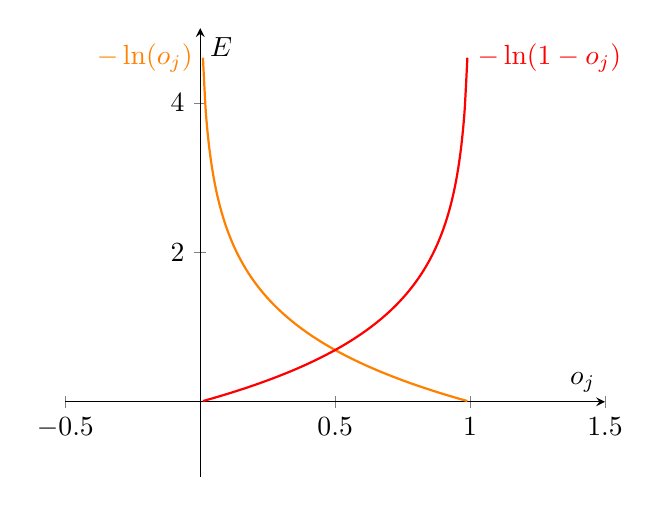
\begin{tikzpicture}
\begin{axis}[
	axis lines = middle,
	xlabel = $o_j$,
	ylabel = $E$,
	ymin = -1,
	ymax = 5,
	xmin = -0.5,
	xmax = 1.5,
	clip = false,
]
\addplot[
	domain = 0:0.99,
	samples = 100, 
	color = orange,
	thick, smooth,
	]
{-ln(x)}
node[left,pos=0] {$-\ln(o_j)$};
\addplot[
	domain = 0.01:1,
	samples = 100, 
	color = red,
	thick, smooth,
	]
{-ln(1-x)}
node[right,pos=1] {$-\ln(1-o_j)$};	
\end{axis}
\end{tikzpicture}
\caption{Error produced for $t_j=1$ (orange) and for $t_j=0$ (red). $o_j$ must be in range $(0,1]$, otherwise the logarithm can be complex or undefined or the error gets rediciously large.}
\end{figure}

\subsection{L1 and L2 Regularization}
Small weights tend to perform better and we can modify the error functions from above to penalize big weight by adding additional error terms.
\begin{itemize}
\item L1 norm: $||\mathbf{w}||_{L1} = \sum_j |\mathbf{w}_j|$
\item L2 norm: $||\mathbf{w}||_{L2} = \sum_j \mathbf{w}_j^2$
\item new error function $E' = E + \alpha_{L1} ||\mathbf{w}||_{L1} + \alpha_{L2} ||\mathbf{w}||_{L2}$
\item new hyperparamaters $\alpha_{L1}$ and $\alpha_{L2}$, optimize on development set
\end{itemize}

\section{Activation Functions}\label{sec:activation-functions}

\subsection{Step Function}
\begin{equation}\label{eq:step_function}
\phi(x) = 
	\begin{cases}
		1 & \text{if}\, x > 0\\
		0 & \text{if}\, x \leq 0
	\end{cases}
\end{equation}
The derivative is always 0.
\begin{figure}
\centering
\begin{tikzpicture}
\begin{axis}[
	axis lines = middle,
	xlabel = $x$,
	ylabel = $y$,
	ymin = -0.5,
	ymax = 1.5,
	xmin = -1,
	xmax = 1,
	clip = false,
]
\addplot[
	color = blue,
	thick
] coordinates {(-1,0)(0,0)(0,1)(1,1)}
node[above,pos=1] {$\phi(x)$};
\end{axis}
\end{tikzpicture}
\caption{Step Function}
\end{figure}

\subsection{Sigmoid}\label{sec:sigmoid}
Most common activation function, can saturate and is easy to dervice.
\begin{equation}\label{ed:sigmoid}
\sigma(x) = \frac{1}{1 + e^{-\beta x}}
\end{equation}
And it's derivative:
\begin{align}\label{ed:sigmoid_derivative}
\begin{split}
\frac{d\,\sigma(x)}{d\,x} &= \frac{d}{d\,x} (1 + e^{-\beta x})^{-1}\\
&= (-1) (1 + e^{-\beta x})^{-2} (-\beta e^{-\beta x})\\
&= \beta (1 + e^{-\beta x})^{-2} e^{-\beta x}\\
&= \beta \frac{1}{1 + e^{-\beta x}} \frac{e^{-\beta x}}{1 + e^{-\beta x}}\\
&= \beta \sigma(x) \frac{e^{-\beta x} + 1 - 1}{1 + e^{-\beta x}}\\
&= \beta \sigma(x) (1 - \frac{1}{1 + e^{-\beta x}})\\
&= \beta \sigma(x) (1 - \sigma(x))
\end{split}
\end{align}
And because there exists algorithm using this, you should have seen the second derivative as well ($\beta=1$):
\begin{align}
\begin{split}
\frac{d\,\sigma(x)(1-\sigma(x))}{d\,x} &= (1-\sigma(x)) \frac{d\,\sigma(x)}{d\,x} + \sigma(x) \frac{d\,(1-\sigma(x))}{d\,x}\\
&= (1-\sigma(x)) \sigma(x) (1 - \sigma(x)) + \sigma(x) (-1) \sigma(x) (1 - \sigma(x))\\
&= \sigma(x) (1 - \sigma(x))^2 - \sigma(x)^2 (1 - \sigma(x))
\end{split}
\end{align}

\begin{figure}
\centering
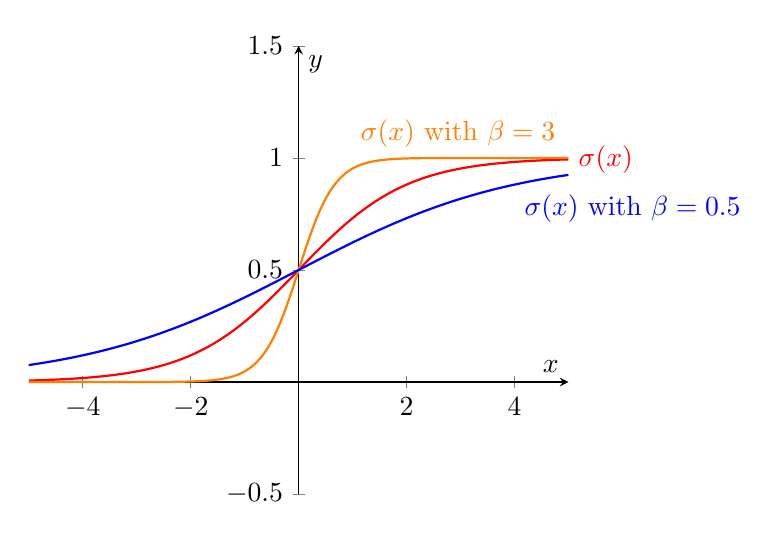
\begin{tikzpicture}
\begin{axis}[
	axis lines = middle,
	xlabel = $x$,
	ylabel = $y$,
	ymin = -0.5,
	ymax = 1.5,
	xmin = -5,
	xmax = 5,
	clip = false,
]
\addplot[
	samples = 100, 
	color = red,
	thick, smooth,
	]
{1/(1+e^(-x))}
node[right,pos=1] {$\sigma(x)$};
\addplot[
	samples = 100, 
	color = orange,
	thick, smooth,
	]
{1/(1+e^(-3*x))}
node[above,pos=0.8] {$\sigma(x)$ with $\beta=3$};
\addplot[
	samples = 100, 
	color = blue,
	thick, smooth,
	]
{1/(1+e^(-0.5*x))}
node[below right,pos=0.9] {$\sigma(x)$ with $\beta=0.5$};
\end{axis}
\end{tikzpicture}
\caption{Sigmoid function with $\beta=1$ (red), $\beta=3$ (orange) and $\beta=0.5$ (blue).}
\end{figure}

\begin{figure}
\centering
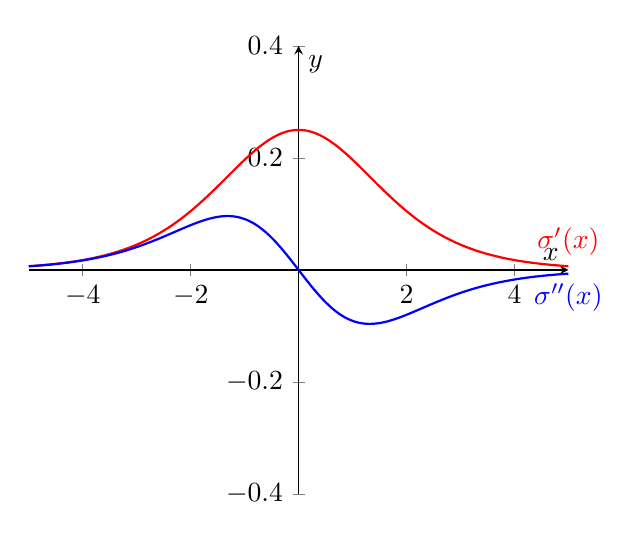
\begin{tikzpicture}
\begin{axis}[
	axis lines = middle,
	xlabel = $x$,
	ylabel = $y$,
	ymin = -0.4,
	ymax = 0.4,
	xmin = -5,
	xmax = 5,
	clip = false,
]
\addplot[
	samples = 100, 
	color = red,
	thick, smooth,
	]
{(1/(1+e^(-x)))*(1-(1/(1+e^(-x))))}
node[above,pos=1] {$\sigma'(x)$};
\addplot[
	samples = 100, 
	color = blue,
	thick, smooth,
	]
{(1/(1+e^(-x)))*(1-(1/(1+e^(-x))))^2 - (1/(1+e^(-x)))^2*(1-(1/(1+e^(-x))))}
node[below,pos=1] {$\sigma''(x)$};
\end{axis}
\end{tikzpicture}
\caption{First and second derivative of the sigmoid function.}
\end{figure}

\subsection{Softmax Function}
In a classification problem we would like $\mathbf{a}$ to be a probability distribution ($\Rightarrow \sum_i a_i = 1$). The softmax function will output a posteriori probability ($p(k|x$) and the biggest value from the layer below is very likely to be close to $1$.
\begin{equation}\label{ed:softmax}
a_i = \phi(z_i) = \frac{e^{z_i}}{\sum_j e^{z_j}}
\end{equation}
And it's derivative:
\begin{align}
\begin{split}\label{ed:softmax_derivative}
\frac{\partial \phi(z_i)}{\partial z_i}
&= \frac{\left(\frac{\partial}{\partial z_i} e^{z_i}\right)(\sum_j e^{z_j}) - e^{z_i} \left(\frac{\partial}{\partial z_i}(\sum_j e^{z_j})\right)}{(\sum_j e^{y_j})^2}\\
&= \frac{e^{y_i} \sum_j e^{y_j} - e^{y_i} e^{y_i}}{(\sum_j e^{y_j})^2}\\
&= \frac{e^{y_i} \sum_j e^{y_j}}{(\sum_j e^{y_j})^2} - \frac{e^{y_i} e^{y_i}}{(\sum_j e^{y_j})^2}\\
&= \frac{e^{y_i}}{\sum_j e^{y_j}} - \left(\frac{e^{y_i}}{\sum_j e^{y_j}}\right)^2\\
&= \phi(y_i) - \phi(y_i)^2\\
&= \phi(y_i) (1 - \phi(y_i))
\end{split}
\end{align}

\subsection{Hyperbolic Tangent Function}
Similar to Sigmoid function, but with outputs in $[-1,1]$. Also not that if the input has a mean of $0$ then so will the output.

\todo{Why is $\tanh$ worth the computational overhead over sigmoid?}
\begin{equation}
\phi(x) = \tanh(x) = \frac{e^x - e^{-x}}{e^x + e^{-x}}
\end{equation}
And it's derivative:
\begin{equation}
\frac{d\phi(x)}{dx} = 1 - \tanh(x) = \frac{(e^x - e^{-x})^2}{(e^x + e^{-x})^2}
\end{equation}
\begin{figure}
\centering
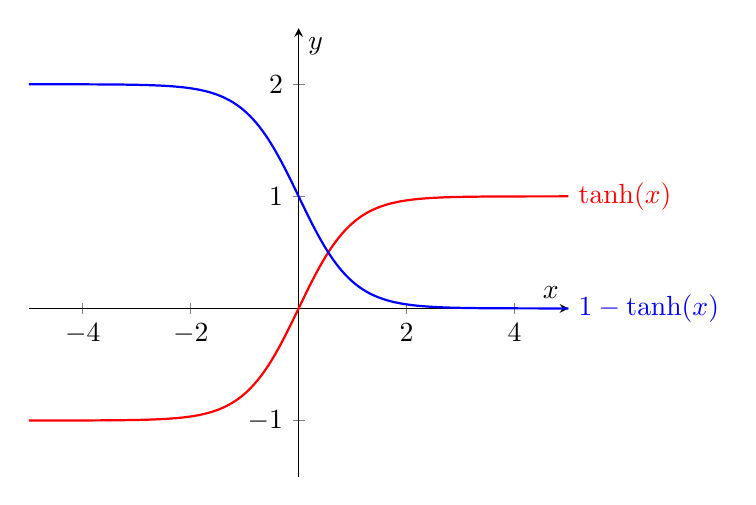
\begin{tikzpicture}
\begin{axis}[
	axis lines = middle,
	xlabel = $x$,
	ylabel = $y$,
	ymin = -1.5,
	ymax = 2.5,
	xmin = -5,
	xmax = 5,
	clip = false,
]
\addplot[
	samples = 100, 
	color = red,
	thick, smooth,
	]
{tanh(x)}
node[right,pos=1] {$\tanh(x)$};
\addplot[
	samples = 100, 
	color = blue,
	thick, smooth,
	]
{1-tanh(x)}
node[right,pos=1] {$1 - \tanh(x)$};
\end{axis}
\end{tikzpicture}
\caption{Hyperbolic Tangent Function (red) and its derivative (blue).}
\end{figure}

\subsection{Linear Function}
Very simple, but with two big downsides. The gradient is always $1$ and multi-layers using it effectively only do a linear combination and therefore can be left out.
$$\phi(x) = x$$

\begin{figure}
\centering
\begin{tikzpicture}
\begin{axis}[
	axis lines = middle,
	xlabel = $x$,
	ylabel = $y$,
	ymin = -5,
	ymax = 5,
	xmin = -5,
	xmax = 5,
	clip = false,
]
\addplot[
	domain = -5:5, 
	samples = 100, 
	color = blue,
	thick, smooth,
	]
{x}
node[left,pos=0] {$x$};
\addplot[
	domain = -5:5, 
	samples = 100, 
	color = red,
	thick, smooth,
	]
{max(0,x)}
node[left,pos=0] {$\max(0,x)$};
\addplot[
	domain = -5:5, 
	samples = 100, 
	color = orange,
	thick, smooth,
	]
{ln(1+e^x)}
node[right,pos=1] {$\ln(1+e^x)$};	
\end{axis}
\end{tikzpicture}
\caption{Linear Function (blue), Rectified Linear Unit (red), Softplus (orange)}
\end{figure}

\subsection{Rectified Linear Unit}
The Rectified Linear Unit (ReLU) is more biologically plausible.
\begin{align}
\phi(x) = \max(0, x)
\intertext{And it's derivative}
\frac{d\phi(x)}{dx} = 
	\begin{cases}
		1 & \text{if}\, x > 0\\
		0 & \text{if}\, x \leq 0\\
	\end{cases}
\end{align}

\subsection{Softplus}
Smoothed version of ReLU.
\begin{align}\label{eq:softplus}
\phi(x) = \ln(1 + e^x)
\intertext{And it's derivative}
\frac{d\phi(x)}{dx} = \frac{e^x}{1 + e^x} = \frac{1}{e^{-x} + 1}
\end{align}

\subsection{Maxout}
Literature: \cite{Goodfellow2013}

Outputs the maximum of its inputs
\begin{equation}
a_j^{(l)} = \max_i z_i^{(l)}, \quad (j-1)g +1 \leq i \leq j g \\
\end{equation}
where $z_i^{(l)} = b^{(l)} + \sum_k w_{ki}^{(l)} x_k^{(l-1)}$ is the summed input and $g$ the size of the group on which we take the maximum.

\section{Learning Rate}\label{sec:learning-rate}
Literature: \cite[Chapter 6.8]{Duda2000}

We use the learning rate $\eta$ in our weight updates: $$w_{ij} \leftarrow w_{ij} + \eta\, \delta_j a_i$$

There are several problems with a constant learning rate:
\begin{itemize}
\item large learning rate
	\begin{itemize}
	\item constantly jump past the minimum ($\Rightarrow$ no convergence)
	\item neurons may saturate
	\end{itemize}
\item small learning rate
	\begin{itemize}
	\item slow training
	\item may get stuck in local minimum
	\end{itemize}
\end{itemize}

And of course several ways to deat with it them:
\begin{itemize}
\item Predetermined piecewise constant learning rate\newline
	Use a predetermined sequence of $\eta_i$, increment $i$ after every iteration (epoch/batch)
\item Exponentially decaying learning rate
\item Performance Scheduling
\item Weight Dependent Learning Rate Methods (\eg Momentum, AdaGrad)
\end{itemize}

\subsection{Exponential Decaying Learning Rate}
We calculate a new learning rate $\eta(t)$ after each iteration (epoch/batch).
\begin{equation}\label{eq:exponential-decaying-eta}
\eta(t)=\alpha\eta(t-1)=\alpha^t\eta(0)
\end{equation}
With the parameter $\alpha \in (0,1)$ and we still have to define an initial learning rate $\eta(0)$.

\subsection{Performance Scheduling}
Measure the cross validation error and decrease the learning rate when the error stops improving.

\subsection{Momentum}\label{sec:momentum}
Similar to a rock rolling down a hill we let our gradient get some momentum to speed up training while the direction (sign) of the gradient stays the same. We do so by modifying our weight update rule to,
\begin{align}\label{eq:momentum}
w_{ij} &\leftarrow w_{ij} + v_{ij}(t)\\
v_{ij}(t) &\coloneqq \alpha\, v_{ij}(t-1) - \eta\, \delta_j a_i^{(l-1)}
\end{align}
, with $\alpha$ as momentum factor.

A lot of research has gone into the question on how to pick/adjust both $\eta$ and $\alpha$, a good start for the discussion is \cite{Yu1997}.

\subsection{Resilient Propagation (Rprop)}\label{sec:rprop}
Literature: \cite{Riedmiller1994}

Same idea as \emph{Momentum} but just a bit more complicated. Only the sign of the gradient $\frac{\partial E(t)}{\partial w_{ij}}$ is used to adjust the values $v_{it}(t)$. It also introduces several new hyperparameters ($v_0$, $v_{\text{min}}$, $v_{\text{max}}$, $\alpha^+$, $\alpha^-$) instead of just one.
\begin{align}
w_{ij} &\leftarrow \begin{cases}
	w_{ij} - v_{ij}(t) & \text{if } \frac{\partial E(t)}{\partial w_{ij}} > 0\\
	w_{ij} + v_{ij}(t) & \text{if } \frac{\partial E(t)}{\partial w_{ij}} < 0
	\end{cases}\\
v_{ij}(0) &= v_0\\
v_{ij}(t) &= \begin{cases}
	\alpha^+ v_{ij}(t-1) & \text{if } \frac{\partial E(t-1)}{\partial w_{ij}} \frac{\partial E(t)}{\partial w_{ij}} > 0\\
	\alpha^- v_{ij}(t-1) & \text{if } \frac{\partial E(t-1)}{\partial w_{ij}} \frac{\partial E(t)}{\partial w_{ij}} > 0\\
	v_{ij}(t-1) & \text{else}
	\end{cases}
\end{align}
In practice the starting weight update $v_0$ should be a small and $v_{ij}(t)$ should be limited to $[v_{\text{min}}, v_{\text{max}}]$. Good values for $\alpha^-$ and $\alpha^+$ are $0.5$ and $1.2$.

\subsection{AdaGrad}
Literature: \cite{Zeiler2012,Duchi2011,Dyer}

AdaGrad alters the weight update to adapt based on historical information, so that frequently occurring features in the gradients get small learning rates and infrequent features get higher ones.

\begin{align}
g_{ij} &= \frac{\partial E}{\partial w_{ij}}\\
\eta_{ij}(t) &= \frac{\eta_0}{\sqrt{\sum_{\tau=1}^t g_{ij}(\tau)^2}}\,g_{ij}(t)\\
w_{ij}(t) &\leftarrow w_{ij}(t-1) - \eta_{ij}(t)\,g_{ij}(t)
\end{align}

This eliminates the hyperparameter $\eta$, but introduces an initial learning rate $\eta_0$ and has some more downsides \cite{Zeiler2012}. One way to improve it is the limit the window for the sum to size $w$.
\begin{equation}
\eta_{ij}(t) = \frac{\eta_0}{\sqrt{\sum_{\tau=1}^w g_{ij}(t-\tau)^2}}\,g_{ij}(t)\\
\end{equation}

\emph{AdaDelta} contains further improvements.

\subsection{Newbob Scheduling}
Combination of exponential decaying learning rate and performance scheduling. Easy to implement and solid results.
\begin{description}
\item[\textbf{Phase 1}] Start with constant learning rate $\eta(0)$
\item[\textbf{Phase 2}] Once the cross-validation error stops decreasing switch to exponential decaying learning rate
\item[\textbf{Terminate}] End training after cross-validation error stops decreasing again
\end{description}

\chapter{Hopfield Nets and Boltzmann Machines}\label{chapter:bm}

\section{Hopfield Nets}\label{sec:hopfield-nets}
Literature: \cite[Chapter 5.5]{Patterson1997}

In the following we will only consider binary Hopfield nets, in which the neurons are limited to states $0$ (or $-/-1$) and $1$ (or $+/+1$) (sometimes also denoted as $+$ and $-$ or $-1$ and $+1$). Hopfield nets are not very efficient, but good to show the principle of neural nets and a good introduction to Boltzmann machines.

Hopfield nets consist of a single layer of neurons, that is fully connected and acts both as input and output layer. Weights are stored an a weight matrix $W$, where the entry $W_{ij}$ correspondents to the connection weight form neuron~$i$ to neuron~$j$. We will not allow self loops ($W_{ii} = 0$) and the connections will be symmetric ($W_{ij}=W_{ji}$). There exists variations without those limitations.

\subsection{Update Procedure}
\begin{enumerate}
\item Set state $x$ to our input
\item Update neuron state using
	$$x_j = \phi\left(\sum_i W_{ij} x_i \right)$$
	where $\phi(z)$ is the step function
	\begin{equation}
	\phi(z) = \begin{cases}
		1 & \text{if } z > 0\\
		0 & \text{if } z \leq 0
	\end{cases}
	\end{equation}

	We have several options which neurons should be updated:
	\begin{itemize}
	\item In parallel (asynchronous)
	\item Sequential in fixed order (synchronous)
	\item Sequential in random order (synchronous, closest match to biological neural nets)
	\item combination of sequential and parallel
	\end{itemize}
\item Repeat step 2 until $x$ stabilizes.
\item State $x$ is our output
\end{enumerate}

\subsection{Energy function}
\begin{equation}
E = -\half \sum_i \sum_{j\neq i} x_i x_j W_{ij}
\end{equation}
This is our objective function that we are going to minimize.

\subsection{Convergence}
If only one neuron~$j$ is updated at the time, the update will always lead to the same or lower energy.
\begin{itemize}
\item $x_j(t+1) = x_j(t) \Rightarrow$ state did not change, energy stays the same
\item $x_j(t+1) = 1 - x_j(t) \Rightarrow$ state did changed, compute the energy change
	\begin{align}
	E_j &= -\half \sum_i x_i x_j W_{ij}\\
	\Delta E &= E_j(t+1) - E_j(t)\\
	&= -\half \left[ x_j(t+1) \sum_i x_i W_{ij} - x_j(t) \sum_i x_i W_{ij} \right]\\
	&= -\half \Delta x_j \sum_i x_i W_{ij}\quad\text{with}\quad	\Delta x_j = x_j(t+1) - x_j(t)\\
	\intertext{Change from 0 to 1}
	\Delta x_j &= 1,\,\sum_i x_i W_{ij} > 0 \Rightarrow \Delta E_j \leq 0\\
	\intertext{Change from 1 to 0}
	\Delta x_j &= -1,\,\sum_i x_i W_{ij} \leq 0 \Rightarrow \Delta E_j \leq 0
	\end{align}
\end{itemize}

\subsection{Training}
\begin{equation}
W_{ij} = \sum_{x \in X} (2x_i -1)(2x_j-1)
\end{equation}

\begin{equation}
W_{ij} = \frac{1}{|X|} \sum_{x \in X} x_i x_j
\end{equation}

\subsection{Associative memory}

\subsection{Limitations}


\section{Boltzmann Machines}\label{sec:bm}
Boltzmann machines are stochastic recurrent neural networks.

Boltzmann machines work similar to Hopfield nets. They have a binary state vector ($x_j \in {0,1}$), but the new state a neuron $x_j$ is determined stochastically (based on the total input $z_j$) on each update of $x_j$.

\begin{equation}
z_j = b_j + \sum_i x_i w_{ij}
\end{equation}
The probability that the activation of neuron $x_j$ is set to $1$ is calculated using the sigmoid function,
\begin{equation}
p(x_j = 1) = \sigma(z_j) = \frac{1}{1 + e^{-z_j}}
\end{equation}
, otherwise the activation of $x_j$ becomes $0$.

In general Boltzmann machines are unrestricted (see \ref{sec:rbm} for \gls{RBM}), but have the properties:
\begin{itemize}
\item Network is fully connected
\item No self connections, $w_{ii}=0$
\item Undirected/symmetric, $w_{ij}=w_{ji}$
\end{itemize}

One can define input neurons that have the fixed input value during evaluation.

\subsection{Energy}
The energy of a state $x$ is defined by
\begin{equation}
E(x) = - \sum_i x_i b_i - \half \sum_{i<j} x_i x_j w_{ij}
\end{equation}

With this we can calculate the probability of a state $x$
\begin{equation}
p(x) = \frac{e^{-E(x)}}{\sum_y e^{-E(y)}}
\end{equation}

In average updating the neurons will decrease the energy in the network.

\subsection{Simulated Annealing}
Use temperature $T$ to allow more changes in the beginning (\eg jumps out of bad local minima) by using the sigmoid function with $\beta=\frac{1}{T}$.
\begin{equation}
p(x_j = 1) = \frac{1}{1 + e^{\frac{-z_j}{T}}}
\end{equation}
Figure \ref{fig:bm-simulated-annealing} shows curves with different temperature.

\begin{figure}
\centering
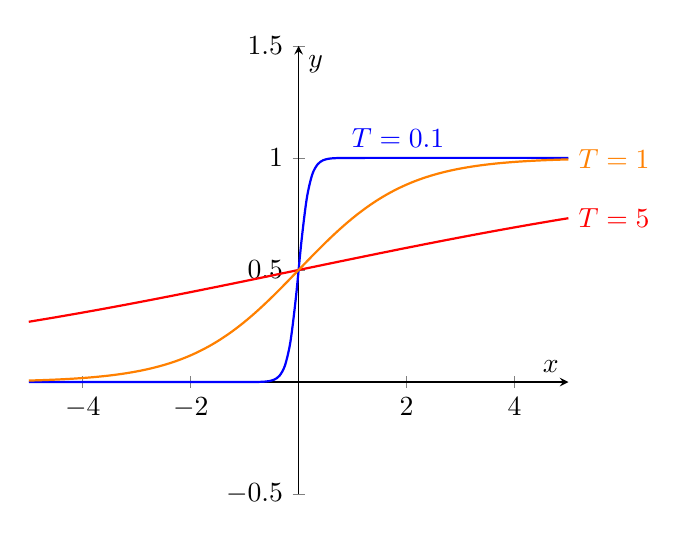
\begin{tikzpicture}
\begin{axis}[
	axis lines = middle,
	xlabel = $x$,
	ylabel = $y$,
	ymin = -0.5,
	ymax = 1.5,
	xmin = -5,
	xmax = 5,
	clip = false,
]
\addplot[
	samples = 100, 
	color = red,
	thick, smooth,
	]
{1/(1+e^(-x/5))}
node[right,pos=1] {$T=5$};
\addplot[
	samples = 100, 
	color = blue,
	thick, smooth,
	]
{1/(1+e^(-x/0.1))}
node[above,pos=0.7] {$T=0.1$};

\addplot[
	samples = 100, 
	color = orange,
	thick, smooth,
	]
{1/(1+e^(-x))}
node[right,pos=1] {$T=1$};
\end{axis}
\end{tikzpicture}
\caption{Sigmoid function (orange), with high temperature (red) and low temperature (blue).}
\label{fig:bm-simulated-annealing}
\end{figure}

\subsection{Why to restrict BMs}
Unrestricted Boltzmann machines are very powerful and can compute every function. But due the complex net structure the training is very slow and computational expensive.




\section{Restricted Boltzmann Machines}\label{sec:rbm}


\chapter{Autoencoders}\label{chapter:da}

\section{Training}

\section{Spares Autoencoders}

\section{Denoising Autoencoders}

\section{Stacking Autoencoders}
%!TEX root = ../NeuralNets.tex
\chapter{Advanced Neural network architectures}

\section{Time Delay Neural Networks (TDNN)}\label{sec:tdnn}

%!TEX root = ../NeuralNets.tex
\section{Multi-State Time Delay Neural Networks (MS-TDNN)}\label{sec:ms-tdnn}\xindex{TDNN}%
Literature: \cite{Haffner1992,Hild1993}

%!TEX root = ../NeuralNets.tex
\section{Convolutional Neural Networks (CNN)}\label{cnn}\xindex{CNN}%


\section{Recurrent Neural networks (RNN)}\label{sec:rnn}

\subsection{Vanishing Gradient}

\subsection{Backpropagation through Time}

\chapter{Practical Tricks}\label{chapter:practical-tricks}

\section{Data Normalization}\label{sec:data-normalization}

Numerical needs to be normalized because \gls{NN} function best with inputs between in range $[0,1]$ or $[-1,+1]$. There are two common normalizations, the min-max normalization (sometimes called feature scaling),
\begin{equation}\label{eq:min_max_normalization}
\hat x_i = \frac{x_i - \min(x)}{\max(x) - \min(x)}
\end{equation}
, which will transform the smallest value to $0$ and the biggest to $1$ and everything else linearly in between, and gaussian normalization,
\begin{equation}\label{eq:gaussian_normalization}
\hat x_i  = \frac{x_i - \text{mean}(x)}{\text{std}(x)} = \frac{x_i - \mu}{\sigma}
\end{equation}
, will transform $x$ to have zero mean and a standard deviation of one. Other names for int are standard score or z-scores.

Those are the two most common methods, but depending on the input there might be more.

\section{Bottleneck-Features}\label{sec:bottleneck-features}

\begin{figure}
\centering
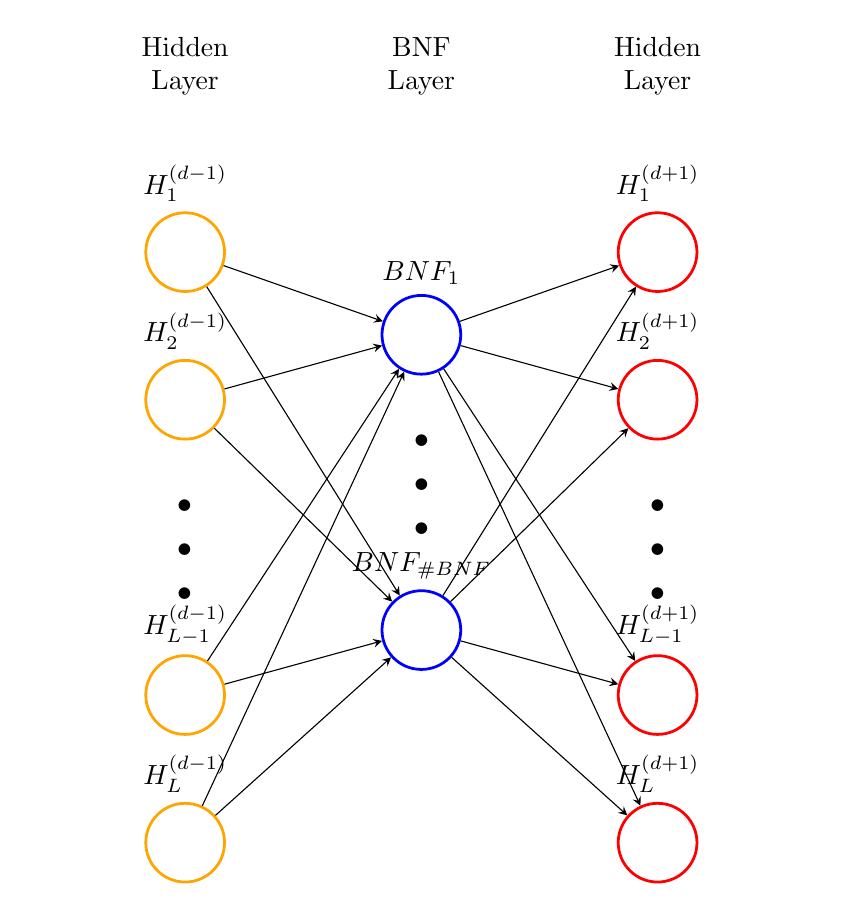
\begin{tikzpicture}[x=1.5cm, y=1.5cm, >=stealth]
% neurons
\foreach \m [count=\y] in {1,2,missing,3,4}
	\node[neuron, neuron-input, neuron-\m/.try ] (hidden1-\m) at (0,2-\y*1.25) {};
\foreach \m [count=\y] in {1,missing,2}
	\node[neuron, neuron-hidden, neuron-\m/.try ] (BNF-\m) at (2,1.3-\y*1.25) {};
\foreach \m [count=\y] in {1,2,missing,3,4}
	\node[neuron, neuron-output, neuron-\m/.try ] (hidden2-\m) at (4,2-\y*1.25) {};

% neuron labels
\foreach \l [count=\i] in {1,2,L-1,...,L-1,L}
	\node[above] at (hidden1-\i.north) {$H^{(d-1)}_{\l}$};
\foreach \l [count=\i] in {1,\#BNF}
	\node[above] at (BNF-\i.north) {$BNF_{\l}$};
\foreach \l [count=\i] in {1,2,L-1,...,L-1,L}
	\node[above] at (hidden2-\i.north) {$H^{(d+1)}_{\l}$};

% neuron connection
\foreach \i in {1,...,4}
	\foreach \j in {1,...,2}
		\draw[->] (hidden1-\i) -- (BNF-\j);
\foreach \i in {1,...,2}
	\foreach \j in {1,...,4}
		\draw[->] (BNF-\i) -- (hidden2-\j);

% layer labels
\foreach \l [count=\x from 0] in {Hidden, BNF, Hidden}
	\node[align=center, above] at (\x*2,2) {\l \\ Layer};

\end{tikzpicture}
\caption{Neural network with Bottleneck features}
\label{fig:bottleneck-features}
\end{figure}


%!TEX root = ../NeuralNets.tex
\section{Weight Decay}\label{sec:weight-decay}
Literature: \cite{Connect1992} and \cite[Chapter 6.8]{Duda2000}

To help generalizing by simplifying a network and to avoid overfitting one can
impose a heuristic that the weights stay small. This may not always lead to
improved network performance, but experience showed that it helps in many cases
and even can be used together with momentum (see \cref{sec:momentum}).

It is also every simple, after each weight update we simply ``decay'' the
weights with a parameter $\epsilon \in (0,1)$.
\begin{equation}\label{eq:weight-decay}
w_{ij} \leftarrow w_{ij} (1-\epsilon)
\end{equation}
combined with the weight update we get
\begin{align}
w_{ij} &\leftarrow (w_{ij} - \eta\, \frac{\partial E}{\partial w_{ij}}) (1-\epsilon)\\
\Delta w_{ij} &= -\epsilon\,w_{ij} - (1-\epsilon)\eta\,\frac{\partial E}{\partial w_{ij}}\\
&= -\epsilon\,w_{ij} - \eta'\,\frac{\partial E}{\partial w_{ij}}\\
&= -\epsilon\,w_{ij} - \eta'\,\frac{\partial E}{\partial w_{ij}}
\end{align}

Those weights that are need to solve the problem will increase enough with the
weight update to compensate the small decrease, but others will get smaller and
smaller until they can be eliminated completely. It can be shown that the above
is equivalent to gradient descent we a modified error function:
\begin{align}
E_{\text{weight decay}} &= E + \frac{2\epsilon}{\eta} \mathbf{w}^T \mathbf{w}
\end{align}



% \bibliographystyle{apalike}
% \bibliography{Remote}

% \printglossary[type=\acronymtype]

\listoftodos

\end{document}